% tikzpic.tex
\documentclass[crop,tikz]{standalone}% 'crop' is the default for v1.0, before it was 'preview'

\usetikzlibrary{arrows,decorations.pathmorphing,decorations.pathreplacing,backgrounds,positioning,fit,matrix}
\usetikzlibrary{shapes,calc,patterns,arrows.meta}
\tikzset{
	vert/.style={circle,inner sep=1.5,fill=white,draw,minimum size=.3cm},
	edge/.style={color=black, thick},
	diredge/.style={->,>={Stealth[width=8pt,length=8pt]},color=black, thick},
	timelabel/.style={fill=white,font=\footnotesize, text centered},
	wave/.style={decorate,decoration={coil,aspect=0}},
	dirwave/.style={->, >={Stealth[width=8pt,length=8pt]},decorate,decoration={coil,aspect=0}},
	diredge2/.style={->,>={Stealth[width=8pt,length=8pt]}}
}
\begin{document}


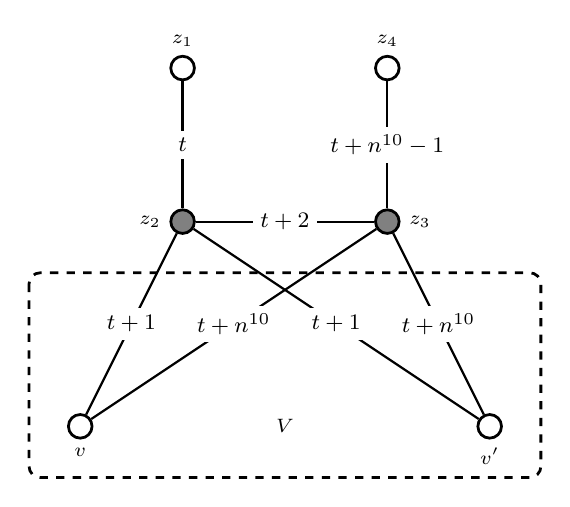
\begin{tikzpicture}[line width=1pt, scale=.65]
	\scriptsize
	
	
	\draw[rounded corners, dashed] (-3, -4) rectangle (7, -8) {};
	\node (A) at (2,-7) {$V$};
	
	\node[vert,label=above:$z_1$] (Z1) at (0,0) {};
	\node[vert,label=left:$z_2$, fill=gray] (Z2) at (0,-3) {};
	\node[vert,label=right:$z_3$, fill=gray] (Z3) at (4,-3) {};
	\node[vert,label=above:$z_4$] (Z4) at (4,0) {};
	
	\node[vert,label=below:$v$] (V) at (-2,-7) {};
	\node[vert,label=below:$v'$] (VV) at (6,-7) {};
	
	\draw[edge] (Z1) --node[timelabel] {$t$} (Z2);
	\draw[edge] (Z2) --node[timelabel] {$t+2$} (Z3);
	\draw[edge] (Z3) --node[timelabel] {$t+n^{10}-1$} (Z4);
	
	\draw[edge] (Z2) --node[timelabel] {$t+1$} (V);
	\draw[edge] (Z3) --node[timelabel] {$t+n^{10}$} (V);
	\draw[edge] (Z2) --node[timelabel] {$t+1$} (VV);
	\draw[edge] (Z3) --node[timelabel] {$t+n^{10}$} (VV);
\end{tikzpicture}

\end{document}